% Important: If latex complains about unicode characters,
% please use "\usepackage[utf8x]{inputenc}" in your preamble
% You can change the size of the picture by putting it into the construct:
% 1) \resizebox{10cm}{!}{"below picture"} to scale horizontally to 10 cm
% 2) \resizebox{!}{15cm}{"below picture"} to scale vertically to 15 cm
% 3) \resizebox{10cm}{15cm}{"below picture"} a combination of above two
% It is not recomended to use the scale option of the tikzpicture environment.
\scalebox{0.98}{
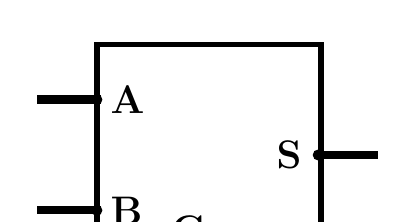
\begin{tikzpicture}[x=1pt,y=-1pt,line cap=rect]
\useasboundingbox (0,0) rectangle (130,60); 
\def\logisimfontA#1{\fontfamily{cmr}{#1}} % Replaced by logisim, original font was "SansSerif"
\def\logisimfontB#1{\fontfamily{CMU Bright}{#1}}
\def\logisimfontC#1{\fontfamily{CMU Sans Serif}{#1}}
\definecolor{custcol_0_0_0}{RGB}{0, 0, 0}
\definecolor{custcol_ff_ff_ff}{RGB}{255, 255, 255}
\draw [line width=3.0pt, custcol_0_0_0 ]  (65.0,86.0) -- (65.0,96.0) ;
\draw [line width=3.0pt, custcol_0_0_0 ]  (5.0,26.0) -- (25.0,26.0) ;
\draw [line width=3.0pt, custcol_0_0_0 ]  (5.0,66.0) -- (25.0,66.0) ;
\draw [line width=3.0pt, custcol_0_0_0 ]  (105.0,46.0) -- (125.0,46.0) ;
\draw [line width=2.0pt, custcol_0_0_0 ]  (25.0,6.0) -- (105.0,6.0) ;
\draw [line width=2.0pt, custcol_0_0_0 ]  (106.0,6.0) -- (106.0,85.0) ;
\draw [line width=2.0pt, custcol_0_0_0 ]  (106.0,86.0) -- (26.0,86.0) ;
\draw [line width=2.0pt, custcol_0_0_0 ]  (25.0,86.0) -- (25.0,7.0) ;
\fontsize{14pt}{14pt}\fontseries{bx}\selectfont\node[inner sep=0, outer sep=0, custcol_0_0_0, anchor=base west] at  (90.0,51.0)  {\textbf{S}};
\fontsize{14pt}{14pt}\fontseries{bx}\selectfont\node[inner sep=0, outer sep=0, custcol_0_0_0, anchor=base west] at  (52.0,78.0)  {\textbf{C$_{out}$}};
\fontsize{14pt}{14pt}\fontseries{bx}\selectfont\node[inner sep=0, outer sep=0, custcol_0_0_0, anchor=base west] at  (30.0,31.0)  {\textbf{A}};
\fontsize{14pt}{14pt}\fontseries{bx}\selectfont\node[inner sep=0, outer sep=0, custcol_0_0_0, anchor=base west] at  (30.0,71.0)  {\textbf{B}};
\fill [line width=1.0pt, custcol_0_0_0]  (25.0,26.0) ellipse (2.0 and 2.0 );
\fill [line width=1.0pt, custcol_0_0_0]  (25.0,66.0) ellipse (2.0 and 2.0 );
\fill [line width=1.0pt, custcol_0_0_0]  (65.0,86.0) ellipse (2.0 and 2.0 );
\fill [line width=1.0pt, custcol_0_0_0]  (105.0,46.0) ellipse (2.0 and 2.0 );
\end{tikzpicture}
}